\documentclass[a4paper, 11pt]{article}
\usepackage[utf8]{inputenc} %interprete de simbolos en español
\usepackage[T1]{fontenc}
\usepackage[spanish]{babel}
\usepackage[margin=2.5cm, top=2.5cm, includefoot]{geometry}
\usepackage{url}
\usepackage{graphicx} % Insercción de imágenes
\usepackage[table,xcdraw]{xcolor} % detección de colores
\usepackage[most]{tcolorbox} % Insercción de cuadros en la portada
\usepackage{fancyhdr} % definir el estilo de la página
\usepackage[hidelinks]{hyperref} % gestión de hipervinculos
\usepackage{listings} % inserccón de codigo 
\usepackage{parskip} % arreglo de tabluación del documento
\usepackage[figurename=Figura]{caption} % cambiar nombre del caption de las fotos
\usepackage{smartdiagram} % insercción de diagramas
\usepackage{zed-csp} % insercción de tablas
\usepackage[scaled]{helvet} % Fuente Helvetica
\usepackage[pages=some]{background} % imagen de fondo
\usepackage{sectsty} 
\usepackage{csquotes} % cargar para asegurar de que los textos citados se componen de acuerdos al idioma principal
\usepackage{tikz}
\usepackage{eso-pic}
\usepackage{stackengine} % opcion1 incluir para poner texto sobre imagen
\usepackage[backend=biber,style=apa,sorting=anyt]{biblatex} % uso de bibliografia
\addbibresource{referencias.bib} % referencia .bib

\renewcommand\familydefault{\sfdefault} % Quitar fuente default

\sectionfont{\fontsize{14}{16.8}\selectfont} % {Tamaño de fuente}{Salto de linea minimo 1.2}
\subsectionfont{\fontsize{12}{14.4}\selectfont}

% Delaracion de Colores
\definecolor{rojoPortada}{HTML}{FF0A0A}

% Delaración de variables
\newcommand{\logoUnivInacap}{imagenes/univ_inacap.png}
\newcommand{\logoInacap}{imagenes/logo_inacap.png}

\newcommand{\fechaEntrega}{\today}
\newcommand{\nombreInforme}{Informe Nombre del trabajo}

% índices
\addto\captionsspanish{\renewcommand{\contentsname}{Índice}} % cambio nombre índice

% Imagen Head
\pagestyle{fancy}
\fancyhf{}
\rhead{\includegraphics[width=8cm]{\logoUnivInacap}}
\fancyfoot[C]{\scriptsize \nombreInforme}
\renewcommand{\headrulewidth}{0pt}

% Propiedades de imagende de fondo
\backgroundsetup{
    angle=0, % en caso de querer una rotación
    scale=1, % escala de la imagen, es recomendable que sea del mismo tamaño que el pdf
    color=black, % fondo a usar para transparencia
    opacity=0.6, % nivel de transparencia
    hshift=5mm,
    vshift=-90mm,
    contents={
        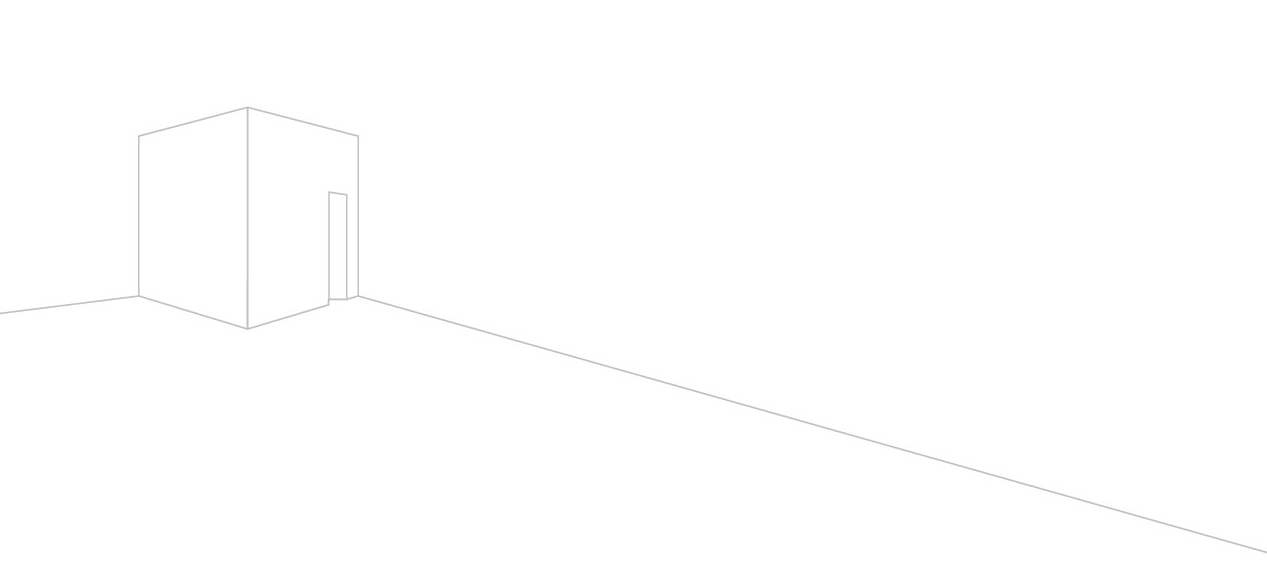
\includegraphics[width=18cm,height=7cm]{imagenes/fondo_portada.png}
    }
}

\begin{document}
    \rfoot[]{\thepage} % número de página lado  derecho

    % Barra superior gris
    \AddToShipoutPictureBG*{
        \AtPageUpperLeft{\color{gray} \rule[-0.8cm]{\paperwidth}{0.6cm}}
    }


    % -- Portada
    \begin{titlepage}

        % Fondo con texto interior.
        \begin{picture}(0,75)
            \stackinset{c}{}{c}{20mm}{\color{white}{\MakeUppercase{\textbf{informática}}}}{
                \stackinset{c}{}{c}{10mm}{\color{white}{\MakeUppercase{\textbf{y telecomunicaciones}}}}{
                    \includegraphics[width=140\unitlength,height=140\unitlength]{\logoInacap}
                }
        }
        \end{picture}

        \vfill

        \begin{center}
            {\Huge\ \textbf{\nombreInforme}\par}
            {\huge\ Nombre de la unidad de aprendizaje\par}                   
        \end{center}

        \vfill
        \vfill

        \textbf{Asignatura: }  "Mi asignatura"\par\vspace{0.3cm}
        \textbf{Sección:} "Mi seccion"\par\vspace{0.3cm}
        \textbf{Nombre del docente:} "Nombre y apellidos"\par\vspace{0.3cm}
        \textbf{Nombre de los integr4antes del grupo: } "Nombres"\par\vspace{0.3cm}

        \vfill
       
        \begin{center}
            \textbf{Fecha de entrega}\par
            \fechaEntrega
        \end{center}
        
        \vfill

        % Imagen de fondo
        \BgThispage

    \end{titlepage}
    \clearpage

    % Barra inferior roja
    \AddToShipoutPictureBG{\color{red}
        \AtPageLowerLeft{\rule{\paperwidth}{1cm}}
    }

    
    % -- Tabla de Contenido
    \tableofcontents
    \clearpage

    % -- Documento
    
    \section{Introducción}
    Presentación de la temática desarrollada en el informe, mediante una página que debe incluir información de manera resumida con respecto a lo que se abordará (se recomienda redactar este apartado al finalizar el cuerpo del informe).
    \clearpage
    
    
    \section{Objetivo}
    Este es un texto de ejemplo en LaTex con nota al pie de página \footcite{latexcompanion}.

    \section{Desarrollo}
    Este es un texto de ejemplo con cita bibliográfica \parencite{latexcompanion}

    \subsection{Item}
    Este es un texto de ejemplo con cita bibliográfica \parencite{knuthwebsite}.

    \subsection{Item}
    Este es un texto de ejemplo con cita bibliográfica \parencite{einstein}.
    \clearpage

    \section{Conclusiones}
    Presentar una síntesis, donde se expongan ideas principales y algunas ideas personales en torno al tema. También puede incorporar ideas fuerza y/o aportes a partir del trabajo desarrollado.También es posible incorporar reflexiones, incluso dejar propuestas de profundización que no fueron posibles de abordar en este informe o trabajo.
    \clearpage

    \section{Bibliografía}
    \printbibliography[title = Referencias]

\end{document}